% Ozanam's sixteen court cards (generated by figs_c1ch12.py).
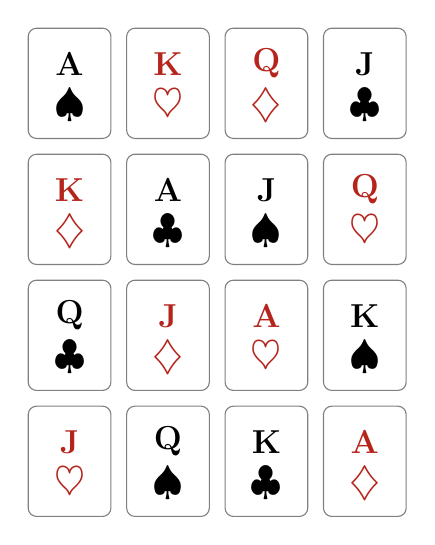
\begin{tikzpicture}[x=1cm,y=1cm]
\draw[rounded corners=3pt,black!50,fill=white] (0.00,-0.00) rectangle (1.05,1.40);
\node[black,font=\large\bfseries] at (0.525,0.950) {A};
\node[black,font=\Large] at (0.525,0.420) {$\spadesuit$};
\draw[rounded corners=3pt,black!50,fill=white] (1.25,-0.00) rectangle (2.30,1.40);
\node[BrickRed,font=\large\bfseries] at (1.775,0.950) {K};
\node[BrickRed,font=\Large] at (1.775,0.420) {$\heartsuit$};
\draw[rounded corners=3pt,black!50,fill=white] (2.50,-0.00) rectangle (3.55,1.40);
\node[BrickRed,font=\large\bfseries] at (3.025,0.950) {Q};
\node[BrickRed,font=\Large] at (3.025,0.420) {$\diamondsuit$};
\draw[rounded corners=3pt,black!50,fill=white] (3.75,-0.00) rectangle (4.80,1.40);
\node[black,font=\large\bfseries] at (4.275,0.950) {J};
\node[black,font=\Large] at (4.275,0.420) {$\clubsuit$};
\draw[rounded corners=3pt,black!50,fill=white] (0.00,-1.60) rectangle (1.05,-0.20);
\node[BrickRed,font=\large\bfseries] at (0.525,-0.650) {K};
\node[BrickRed,font=\Large] at (0.525,-1.180) {$\diamondsuit$};
\draw[rounded corners=3pt,black!50,fill=white] (1.25,-1.60) rectangle (2.30,-0.20);
\node[black,font=\large\bfseries] at (1.775,-0.650) {A};
\node[black,font=\Large] at (1.775,-1.180) {$\clubsuit$};
\draw[rounded corners=3pt,black!50,fill=white] (2.50,-1.60) rectangle (3.55,-0.20);
\node[black,font=\large\bfseries] at (3.025,-0.650) {J};
\node[black,font=\Large] at (3.025,-1.180) {$\spadesuit$};
\draw[rounded corners=3pt,black!50,fill=white] (3.75,-1.60) rectangle (4.80,-0.20);
\node[BrickRed,font=\large\bfseries] at (4.275,-0.650) {Q};
\node[BrickRed,font=\Large] at (4.275,-1.180) {$\heartsuit$};
\draw[rounded corners=3pt,black!50,fill=white] (0.00,-3.20) rectangle (1.05,-1.80);
\node[black,font=\large\bfseries] at (0.525,-2.250) {Q};
\node[black,font=\Large] at (0.525,-2.780) {$\clubsuit$};
\draw[rounded corners=3pt,black!50,fill=white] (1.25,-3.20) rectangle (2.30,-1.80);
\node[BrickRed,font=\large\bfseries] at (1.775,-2.250) {J};
\node[BrickRed,font=\Large] at (1.775,-2.780) {$\diamondsuit$};
\draw[rounded corners=3pt,black!50,fill=white] (2.50,-3.20) rectangle (3.55,-1.80);
\node[BrickRed,font=\large\bfseries] at (3.025,-2.250) {A};
\node[BrickRed,font=\Large] at (3.025,-2.780) {$\heartsuit$};
\draw[rounded corners=3pt,black!50,fill=white] (3.75,-3.20) rectangle (4.80,-1.80);
\node[black,font=\large\bfseries] at (4.275,-2.250) {K};
\node[black,font=\Large] at (4.275,-2.780) {$\spadesuit$};
\draw[rounded corners=3pt,black!50,fill=white] (0.00,-4.80) rectangle (1.05,-3.40);
\node[BrickRed,font=\large\bfseries] at (0.525,-3.850) {J};
\node[BrickRed,font=\Large] at (0.525,-4.380) {$\heartsuit$};
\draw[rounded corners=3pt,black!50,fill=white] (1.25,-4.80) rectangle (2.30,-3.40);
\node[black,font=\large\bfseries] at (1.775,-3.850) {Q};
\node[black,font=\Large] at (1.775,-4.380) {$\spadesuit$};
\draw[rounded corners=3pt,black!50,fill=white] (2.50,-4.80) rectangle (3.55,-3.40);
\node[black,font=\large\bfseries] at (3.025,-3.850) {K};
\node[black,font=\Large] at (3.025,-4.380) {$\clubsuit$};
\draw[rounded corners=3pt,black!50,fill=white] (3.75,-4.80) rectangle (4.80,-3.40);
\node[BrickRed,font=\large\bfseries] at (4.275,-3.850) {A};
\node[BrickRed,font=\Large] at (4.275,-4.380) {$\diamondsuit$};
\end{tikzpicture}
